\section{Quantum Electrodynamics}
We've finally got to QED - the most successful theory in the history of science. All the things we have learned about thus far come into a model that has predictive power - one that predicts things to good accuracy, and experiments can check the results which are very good!

\subsection{Generating Functional for QED}

We want to analyze QED as a QFT. You might guess from what we have done thus far that there might be a generating function of some kind which we can write as a functional integral:
\begin{equation}
    Z[J] = \frac{\int dA d\psi d\bar{\psi} e^{-iS + i \int J^\mu A_\mu + i\int (\bar{\eta}\psi + \bar{\psi}\eta)}}{\int dA d\psi d\bar{\psi}e^{iS}}
\end{equation}
For this coupled theory, we may expect that we have the same structure of deriving the EOMs from the action $S$. This is generally true unless $S$ has a complex canonical structure. We can then use the EOM to derive a functional differential equation for the generating functional, and then we argued that $Z[J]$ solves this with the correct boundary conditions etc. So, a good first guess would be that for any theory, the above is more or less correct. And you would be almost right in proceeding this way. Why almost? Recall that the action for the Maxwell theory is:
\begin{equation}
    S = \int d^4x \left(-\frac{1}{4}F_{\mu\nu}F^{\mu\nu} - i\bar{\psi}(\dirac + m)\psi + e\bar{\psi}\slashed{A}\psi \right)
\end{equation}
where the first term represents the photon field and the second term represents the dirac field, but in our case let's just call it the electron. The third term represents the coupling of the two. Also, notationally recall that $\dirac \equiv \gamma^\mu \p_\mu$. 

If we dropped the interaction term, we would have an exact solution. With the interaction term, there is no analytical solution, and basically the only tool we have is perturbation theory (or numerics - but this has its own difficulties, e.g. the sign problem with the dirac field). For QED, perturbation theory is very useful. Why? Perturbation theory is in $\alpha = \frac{1}{137}$ the fine structure constant, which is very small. So corrections are on the $1\%$ level! This is pretty good convergence. It was said in the old days that QED is for all intents and purposes exactly solved by PT. 

Slight philosophical point - If somehow the actual field theory doesn't exist, then we can just say the PT exists and be happy with that. There are some arguments that the PT is asymptotic - the expansion is singular in $e^2 = 0$. One can make a rough estimate of its convergence; $\alpha = \frac{1}{137}$ and at some order $n$ in PT we have $n!$ Feynman diagram, so we have $\alpha^n n!$ and this starts to inevitably grow because a factorial grows faster than a power. This is about $\sim 100$ terms. That's a lot - we've really only got to 4/5 orders of $\alpha$ done in the literature, and we still have 95 orders to go. Note the fact that the expansion is asymptotic limits the accuracy - but here it is very good.

Other comments - if we started working, then we would see that the electrons are fermions, and $\psi, \bar{\psi}$ are anticommuting variables (which are not really scalars, but some kind of algebraic object). From the assignment you should be aware that we can do Gaussian integrals in terms of such variables. Hence we can apply Wick's theorem.

There is another comment - when solving Maxwell's equation, we fix a gauge. We've written down the gauge invariant form here, but we can't get away with this, even in PT. We are really treating $A$ as the fundamental object here - in the quantum theory we need it. $F_{\mu\nu}F^{\mu\nu}$ is a quadratic form in $A$, and not invertible (the quadratic form has a zero eigenvalue coming from gauge invaraince, so the determinant is zero and so not invertible)... so we need to do something or the two point function does not exist! In summary:
\begin{enumerate}
    \item $\psi, \bar{\psi}$ are anti-commuting
    \item We need to fix a gauge.
\end{enumerate}
So we can't just plug in the action and go ahead with things, and this is generally true for gauge theories. 

\subsection{Fixing the Gauge}
Recalling our discussion of the photon field, we wrote down a relativistic gauge condition:
\begin{equation}
    \p_\mu A^\mu(x) = 0.
\end{equation}
This does fix things, but we need to know how to impose it. In the discussion of the photon field it came in as the physical state condition... but this is not very convenient here. This is because after fixing the gauge, we will want to do PT where the basic ingredient is two point functions. We want to deal with:
\begin{equation}
    \bra{0}TA_\mu(x)A_\nu(x)\ket{0}
\end{equation}
but this is not necessarily physical. What do we do about it? We just ignore it. How do we get away with this? We will agree amongst ourselves that at the end of the day we will only calculate expectation values of gauge invariant quantities. We can check that $F_{\mu\nu}$ will not create unphysical states if we agree to this.

So, our action should be a gauge-fixed one:
\begin{equation}
    S = \int d^4x \left(-\frac{1}{2}\p_\mu A^\nu \p^\mu A_\nu - i\bar{\psi}(\dirac + m)\psi - e\bar{\psi}\slashed{A}\psi\right)
\end{equation}

So we plug this in. But the other terms in the exponential in the generating functional are not gauge invariant. But this is ok as long as we, again, agree to only take expectation values of gauge invariant operators. This sounds awful, and it is because most gauge invariant operators are composites. Another thing that is gauge invariant is the S-matrix (which takes some work to prove) but we could go ahead and calculate S-matrix elements, which is a very useful thing as we do many QED scattering experiments. If this all sounds fuzzy, then that's because it is - most field theorists have a similarly fuzzy understanding of this. And it all seems to work, regardless. Cavalier calculations seem to work out just fine (e.g. giving the photon a small mass...)

Now, we know how to do Gaussian integrals, so we can expand in $e$, get correlators, and we really only need to know functional integration to get to Wick's theorem which gives us a concrete calcualtional tool. However there is still one thing we want to discuss. We have a gauge fixed action, which we plug in. The measure in the functional integral $d\psi, d\bar{\psi}, dA$ are still invariant under gauge transformation (a phase transformation of $\psi, \bar{\psi}$ - here the phases cancel, and a translation of $A$).  Note there is a way to come back to a gauge invariant $S$ from the gauge fixed version - and this will be something useful to do, as we will want to change the gauge fixing condition.

How to do this? We insert $1$ into the generating functional integral:
\begin{equation}
    1 = \int d\Lambda(x)\delta(\p_\mu (A^\mu(x) + \p^\mu \chi(x)) - f(x))\det(-\p^2)
\end{equation}
where we integrate over all gauge transformations. If we plug this into the gauge invariant version of the action, everything is gauge invariant (the measure, the action... forget the sources for now, we can reintroduce them later). The only thing that differes between the two (upon inserting the above) is just the infinite volume factor corresponding to the space of all gauge transformations. If $f = 0$, it is exactly going back and forth between a gauge fixed and invariant action. However, the integral does not depend on $f$, we can multiply and divide by:
\begin{equation}
    x\int df e^{-\frac{\xi}{2}\int f^2(x)dx}
\end{equation}
this integral is just a constant, so we just multiply by a constant. This has the effect inside of the action of introducing a gauge fixing term:
\begin{equation}
    S = \int d^4x \left(-\frac{1}{2}\p_\mu A^\nu \p^\mu A_\nu - i\bar{\psi}(\dirac + m)\psi - e\bar{\psi}\slashed{A}\psi + \frac{\xi}{2}(\p_\mu A^\mu)^2\right)
\end{equation}

Note the determinant $\det(-\p^2)$ has a nice interpretation (though it does not depend on the fields, so it is just another poorly defined infinite constant). When we do fermionic gaussian integrals, the determinant of the quadratic form comes into the numerator - so we can think of that as what is happening here.
\begin{equation}
    \det(-\p^2) = \int d\bar{c}dc e^{-\int \p_\mu \bar{c}\p^\mu c}
\end{equation}
these are known as ghost fields. They decouple from things in QED and we can forget about them, but when we quantize Yang-Mills they stay coupled and we have to consider them. They are never physical, because they violate spin-statistics (spin-0, but they are fermions) and they also have negative metric. We'll forget about the ghots, but we still have the $\frac{\xi}{2}(\p_\mu A^\mu)$ term.

So, the action we use is this gauge fixed object:
\begin{equation}
    S = \int d^4x \left(-\frac{1}{4}F_{\mu\nu}(x)F^{\mu\nu}(x) - \frac{\xi}{2}(\p_\mu A^\mu)^2 - i\bar{\psi}(\dirac + m)\psi + e\bar{\psi}\slashed{A}\psi\right)
\end{equation}
The $\xi$ can be used as a consistency check, but in general people just pick a convenient value.

\subsection{Free-Field Photon and Electron 2-Point Functions}
In the free field theory, we have:
\begin{equation}
    \Delta_{\mu\nu}(x, y) = \bra{0}TA_\mu(x)A_\nu(y)\ket{0}_{e = 0}
\end{equation}
as usual, we know it's Fourier transform:
\begin{equation}
    \Delta_{\mu\nu}(x, y) = \int \frac{d^4k}{(2\pi)^4}e^{ik_\mu (x - y)^\mu}\left(\frac{-i\eta_{\mu\nu}}{k^2 - i\e} - i\left(\frac{1}{\xi} - 1\right)\frac{k_\mu k_\nu}{(k^2 - i\e)^2}\right)
\end{equation}
Where there are now various Gauges we can pick. $\xi = \infty$ is the Landau gauge, $\xi = 1$ the Feynman gauge, $\xi = \frac{1}{3}$ the Kondo-Nakatani gauge etc. In general we can just choose a convenient value for it, as physics should not depend on its value.

There is a slight modification of this theory that has to be done if you have to calculate an S-matrix. That is an infrared regulator:
\begin{equation}
    -\frac{\kappa^2}{2}A_\mu A^\mu
\end{equation}
which we add to the action. If we add that, we should invert the quadratic form with this extra term. In this case, we have the free-field photon propagator:
\begin{equation}
    \Delta_{\mu\nu}(k) = -i\left(\frac{\eta_{\mu\nu} - k_\mu k_\nu / k^2}{k^2 + \kappa^2 - i\e} + \frac{k_\mu k_\nu /k^2}{\xi k^2 + \kappa^2 - i\e}\right)
\end{equation}
and also the electron two-point function:
\begin{equation}
    g_{ab}(x, y) = \bra{0}T\psi_a(x)\bar{\psi}_b(y)\ket{0}_{e=0} = \int \frac{d^4k}{(2\pi)^4} e^{ik_\mu (x - y)^\mu} \frac{[i\slashed{k} - m]_{ab}}{k^2 + m^2 - i\e}
\end{equation}

\subsection{Wick's Theorem}
We have:
\begin{equation}
    \begin{split}
        &\frac{\int dAd\psi d\bar{\psi} e^{iS} A_{\mu_1}(x_1) \ldots A_{\mu_n}(x_n)\psi_{a_1}(y_1) \ldots \psi_{a_m}(y_m) \bar{\psi}_{b_1}(z_1) \ldots \bar{\psi}_{b_k}(z_k)}{\int dA d\psi d\bar{\psi} e^{iS}} 
        \\ &= \sum_{\text{pairings}} (-1)^{\#} \prod_{\text{pairs}}\Delta_{\mu, \nu}(x_i, x_j) g_{a_k, b_l}(y_k, z_l) = 0 \begin{cases}
            \text{if \# $A$s is odd}
            \\ \text{if \# $\psi$s $\neq$ $\bar{\psi}$s}
        \end{cases}
    \end{split}
\end{equation}
Note the $(-1)^{\#}$ comes from the interchanges required to get the fields in the paired form as the fields are anticommuting.

This is what we need to know to start doing PT. From here, we can start to develop Feynman rules. It will be more complicated than scalar field theory PT as we have more indices (but this is a trivial complication).

\subsection{Feynman Diagrams}
The Feynman diagrams are:

\begin{center}
    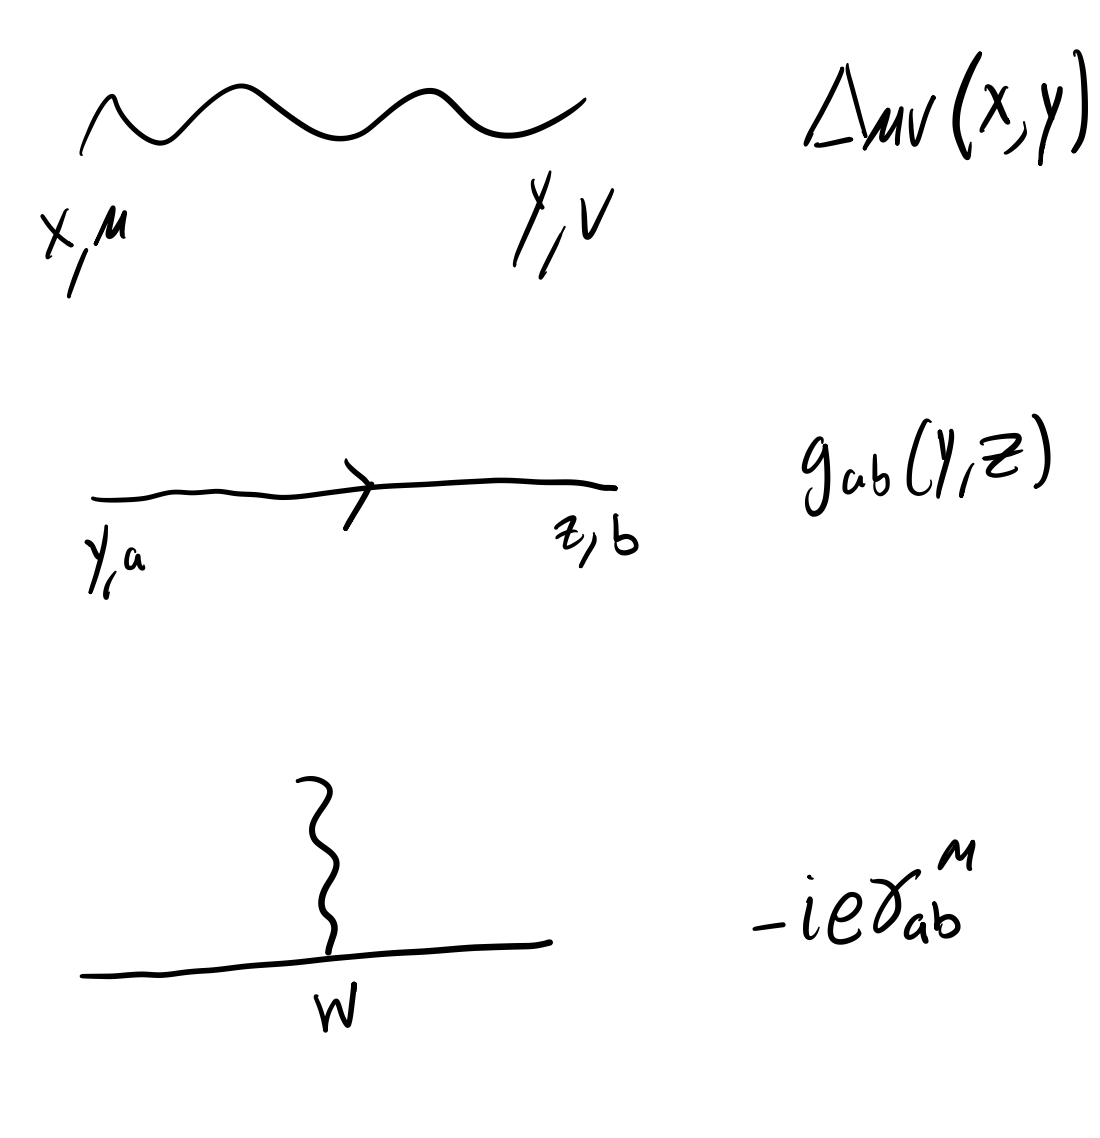
\includegraphics[scale=0.5]{Images/fig-lec31p1.png}
\end{center}

Which are not in principle not more complex than the scalar field case. There are also combinatorial factors that we had in scalar field theory - but in QED, actually these all cancel! So if you don't get a $1$ when doing things explicitly, something has gone wrong. The reason for this has to do with the fact that there is no internal symmetry in the Feynman diagrams.

So, we could generalize what we know already and go to work. But there are a few things to remember here.
\begin{enumerate}
    \item Goldstone's theorem - drop vacuum diagrams (diagrams which have subdiagrams that are not connected to external lines). Like in the case of scalar fields, their contribution is cancelled by the denominator in the functional integral. Does it correspond to the physical interpretation happening? Mathematically it does cancel out.
    \begin{center}
        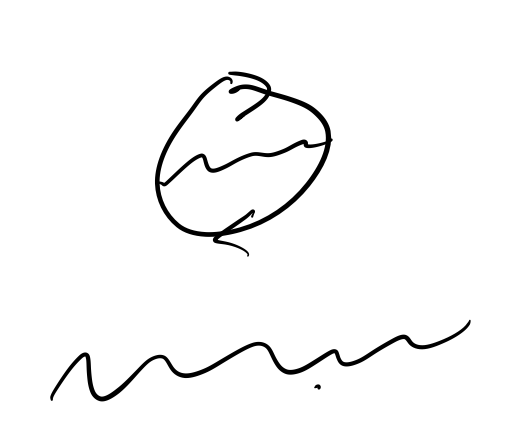
\includegraphics[scale=0.5]{Images/fig-lec31p2.png}
    \end{center}
    \item Furry's Theorem - drop any diagram with a subdiagram emitting an odd number of photons from an electron loop. 
    \begin{center}
        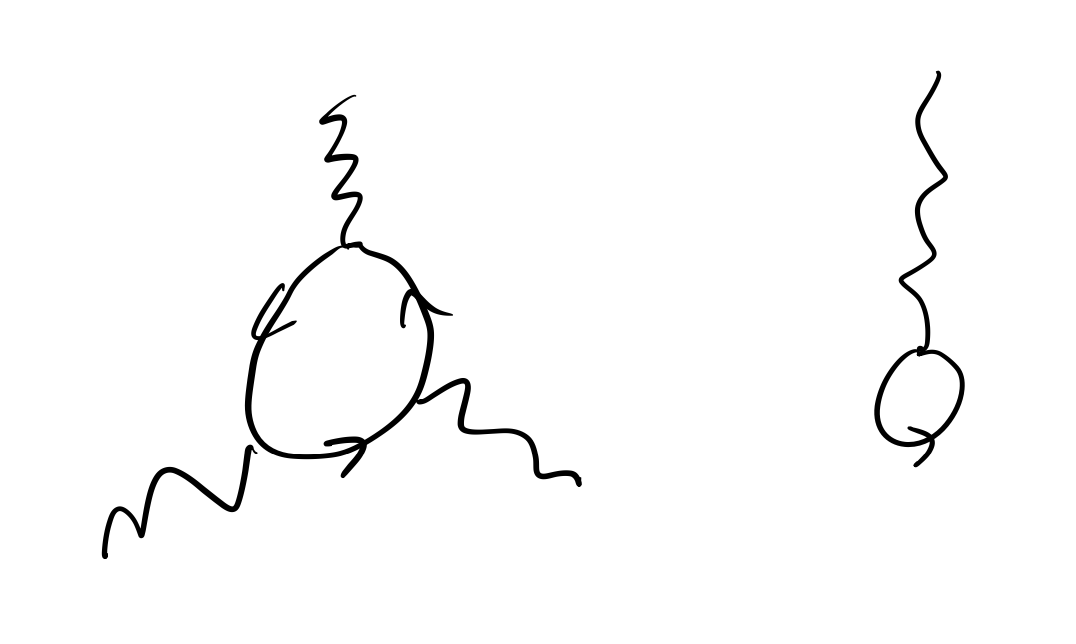
\includegraphics[scale=0.5]{Images/fig-lec31p3.png}
    \end{center}
    the one on the right we could also argue via lorentz invariance. But Furry's theorem also tells us that it vanishes.
    \item Combinatorics - can only be $\pm 1$. $-1$ if we have a closed fermion loop. 
\end{enumerate}

\subsection{Photon 2-Point Function}
For order $e = 0$, we just have free field theory:

\begin{center}
    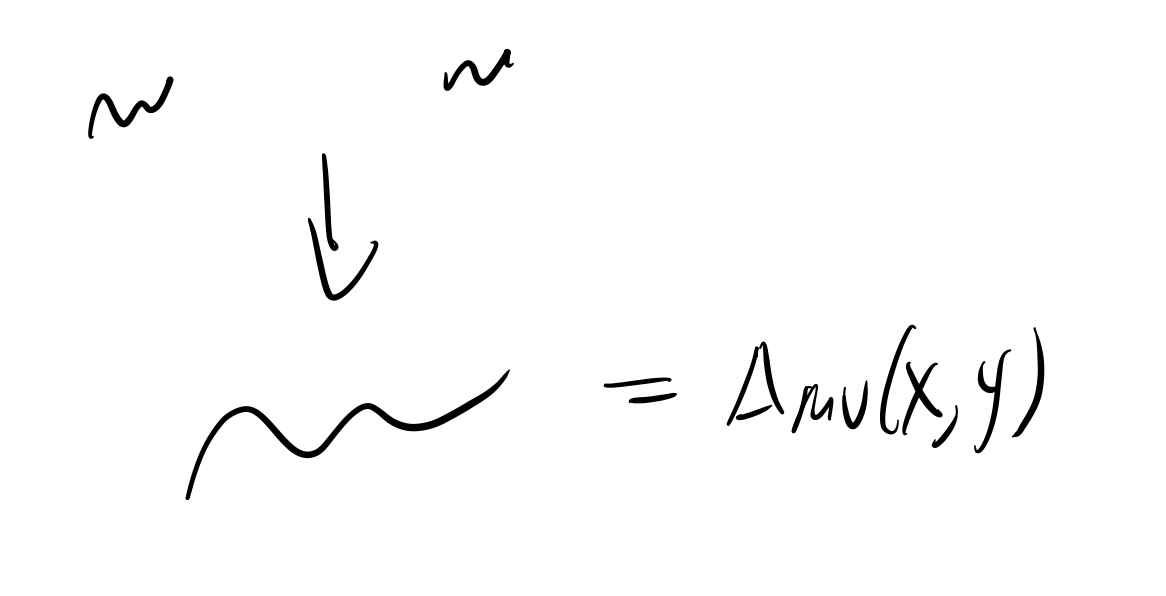
\includegraphics[scale=0.5]{Images/fig-lec31p4.png}
\end{center}

At the moment let us not worry about counterterms and renormalization constants. Now, let's look at higher order. If we look at one vertex (order $e$):

\begin{center}
    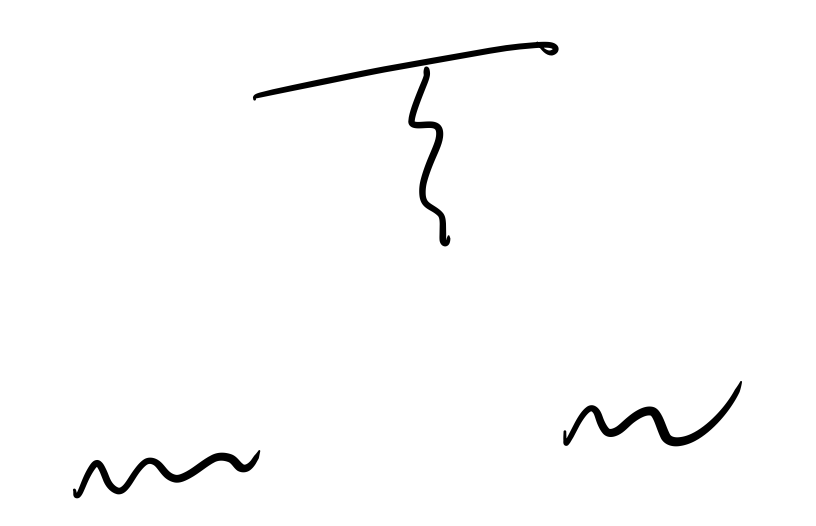
\includegraphics[scale=0.5]{Images/fig-lec31p5.png}
\end{center}

There is no way to pair up all of the legs. So this has no contribution (this would be the case in Wick's theorem of having 3 $A$s). So we look to the next order (order $e^2$) with two vertices:

\begin{center}
    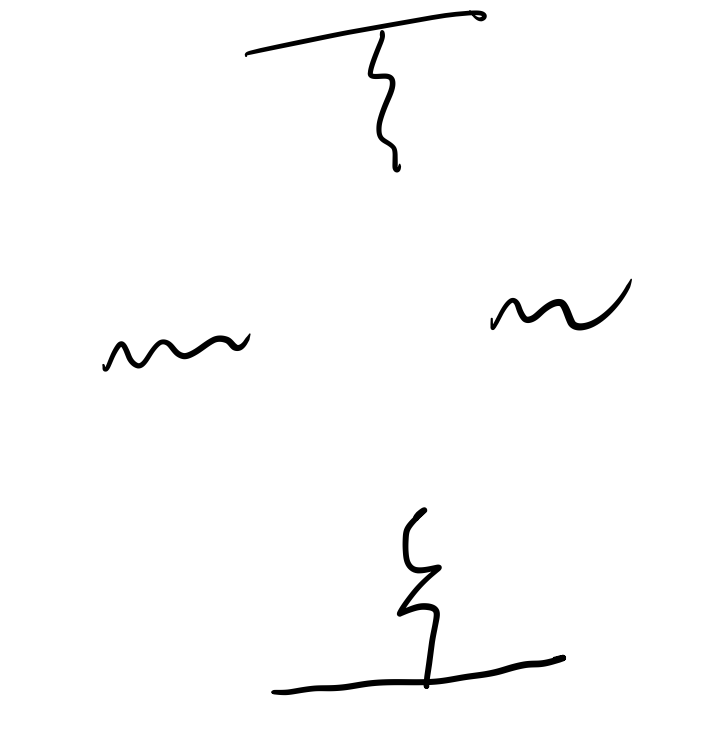
\includegraphics[scale=0.5]{Images/fig-lec31p6.png}
\end{center}

from which we get many things that don't contribute, like:

\begin{center}
    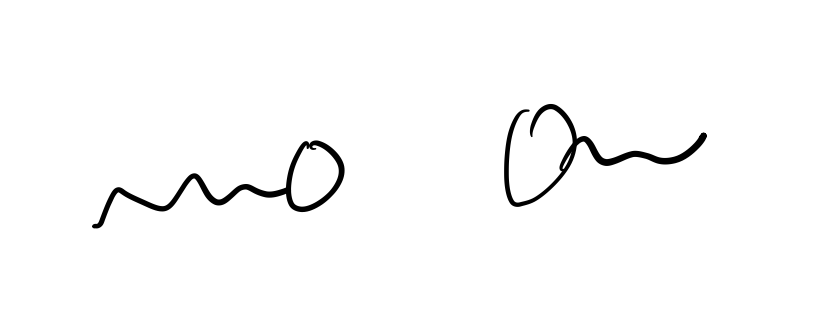
\includegraphics[scale=0.5]{Images/fig-lec31p7.png}
\end{center}

which vanishes via Furry's theorem. Aside from counter-terms, there is only one that contributes:

\begin{center}
    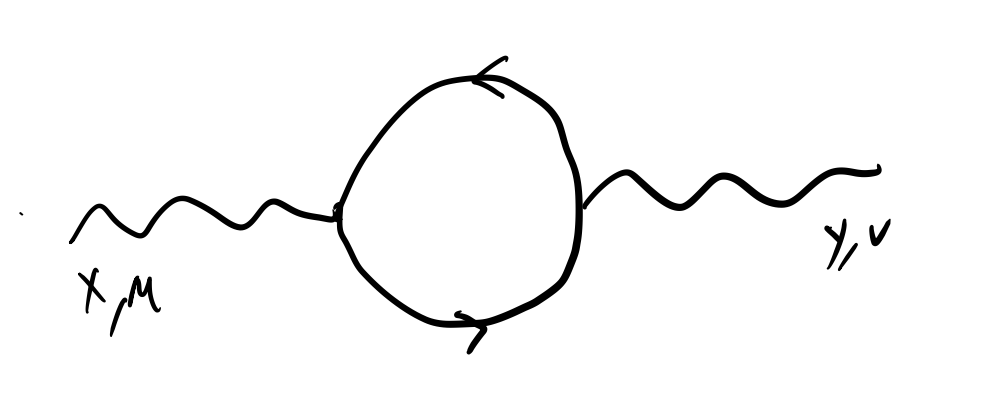
\includegraphics[scale=0.5]{Images/fig-lec31p8.png}
\end{center}

This is connected, and it is close to irreducible (save for the attached internal legs). So we have the Feynman diagram, and from it we can write down the Feynman integral:
\begin{equation}
    \int dw dz (-1)(-ie)^2 \Delta_{\mu\rho}(x, z)\gamma^\rho_{ab}g_{bc}(z, w)\gamma^\sigma_{cd}g_{da}(w, z)\Delta_{\sigma\nu}(w, y)
\end{equation}
note there is no combinatorial factor; the $\frac{1}{2!}$ cancels with the two ways we can form the loop. The minus sign comes from the fact that we have a closed fermion loop. Also, note that all dirac indices are all paired up and summed over, and this makes sense because the photon (the external legs) does not have dirac indices. This looks like a trace of a matrix product.

We can now go to momentum space. Generally there is not a way to do Feynman integrals in position space; so we go to momentum. Let us call the full two-point function $D_{\mu\nu}(k)$. In momentum space, we have:
\begin{equation}
    D_{\mu\nu}(k) = \Delta_{\mu\nu}(k) + e^2 \Delta_{\mu\rho}(k) \int \frac{d^4l}{(2\pi)^4}\Tr(\gamma^\rho g(l)\gamma^\rho g(l+k))\Delta_{\sigma\nu}(k)
\end{equation}
Here, we can see that the $\gamma^\rho g(l)\gamma^\rho g(l+k)$ is the irreducible part and the $\Delta$s are the photon propogators that are trivially attached. The thing to calculate is the central integral which is the irreducible part. In momentum space, we could have written the diagram in a way with different labels:

\begin{center}
    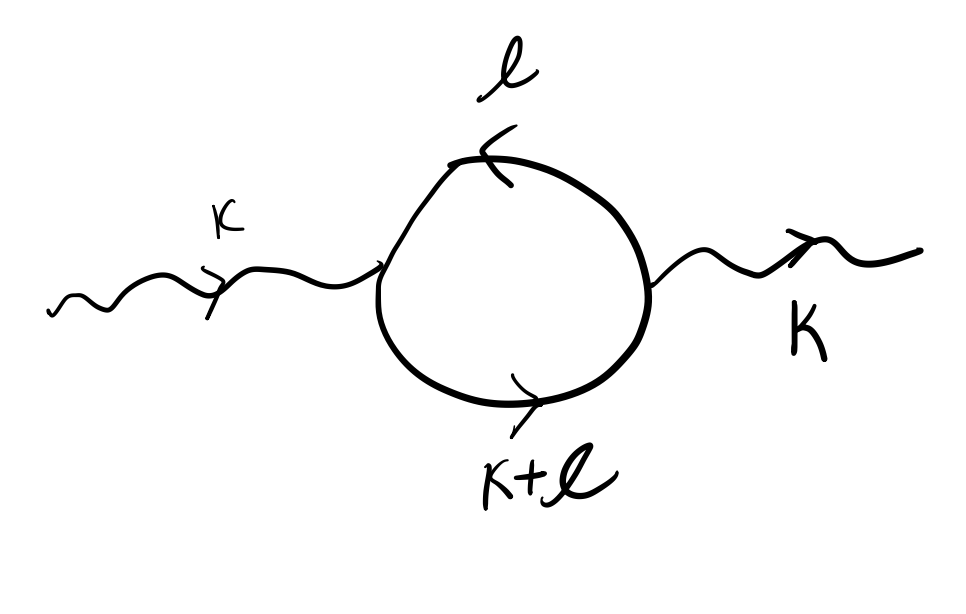
\includegraphics[scale=0.5]{Images/fig-lec31p9.png}
\end{center}
